\uuid{653s}
\chapitre{Autre}
\sousChapitre{Autre}
\titre{ Réseau de neurones multicouches }
\theme{réseaux de neurones}
\auteur{ Maxime NGUYEN }
\datecreate{2024-11-17}
\organisation{ AMSCC }

\contenu{

\question{ Décrire ce que permet de réaliser ce réseau de neurones :


\begin{center}
	\begin{tikzpicture}[scale=1.5]
		\def\layersep{2cm}
		\tikzstyle{every pin edge}=[thick]
		\tikzstyle{neuron}=[circle,fill=black!25,minimum size=12pt,inner sep=0pt]
		\tikzstyle{entree}=[];
		\tikzstyle{input neuron}=[neuron, fill=green!50];
		\tikzstyle{output neuron}=[neuron, fill=red!50];
		\tikzstyle{hidden neuron}=[neuron, fill=blue!50];
		\tikzstyle{annot} = [text width=4em, text centered]
		
		
		% Entree
		\node[entree,blue] (E-1) at (-\layersep,-0.5) {$x$};
		\node[entree,blue] (E-2) at (-\layersep,-2.5) {$y$};
		
		
		% Premiere couche
		\node[input neuron] (I-1) at (0,0) {};
		\node[input neuron] (I-2) at (0,-1.5) {};
		\node[input neuron] (I-3) at (0,-3) {};
		
		
		\node[above right=0.8ex,scale=0.7] at (I-1) {$H$};
		\node[above right=0.8ex,scale=0.7] at (I-2) {$H$};
		\node[below right=0.8ex,scale=0.7] at (I-3) {$H$};
		
		
		\node[below right=0.8ex,scale=0.7] at (I-1) {};
		\node[below right=0.8ex,scale=0.7] at (I-2) {};
		\node[below right=0.8ex,scale=0.7] at (I-2) {};
		
		
		% \node[above right=0.8ex,blue] at (I-1) {$s_1$};
		% \node[above right=0.8ex,blue] at (I-2) {$s_2$};
		% \node[above right=0.8ex,blue] at (I-3) {$s_3$};
		
		
		%Seconde couche et sortie
		\node[output neuron] (O) at (\layersep,-1.5 cm) {};
		\node[below right=0.8ex,scale=0.7] at (O) {};
		\node[above right=0.8ex,scale=0.7] at (O) {$H$};
		
		
		% Arrete et poids
		\path[thick] (E-1) edge node[pos=0.8,above,scale=0.7]{$-1$} (I-1) ;
		\path[thick] (E-2) edge node[pos=0.8,above left,scale=0.7]{$2$} (I-1);
		\draw[-o,thick] (I-1) to node[midway,below right,scale=0.7]{$0$} ++ (-110:0.8);
		
		
		\path[thick] (E-1) edge node[pos=0.8,above,scale=0.7]{$1$} (I-2);
		\path[thick] (E-2) edge node[pos=0.8,above,scale=0.7]{$1$} (I-2);
		\draw[-o,thick] (I-2) to node[midway,below right,scale=0.7]{$-2$} ++ (-130:0.8);
		
		
		\path[thick] (E-1) edge node[pos=0.9,above right,scale=0.7]{$0$} (I-3);
		\path[thick] (E-2) edge node[pos=0.8,above,scale=0.7]{$-1$} (I-3);
		\draw[-o,thick] (I-3) to node[midway,below right,scale=0.7]{$3$} ++ (-130:0.8);
		
		
		\path[thick] (I-1) edge node[pos=0.8,above,scale=0.7]{$1$} (O);
		\path[thick] (I-2) edge node[pos=0.8,below,scale=0.7]{$1$}(O);
		\path[thick] (I-3) edge node[pos=0.8,below,scale=0.7]{$1$}(O);
		\draw[-o,thick] (O) to node[midway,below right,scale=0.7]{$-3$} ++ (-110:0.8) ;
		
		
		% Sortie
		\draw[->,thick] (O)-- ++(1,0) node[right,blue]{$F(x,y)$};
		
		
	\end{tikzpicture}  
\end{center} }


\reponse{This neural network has three neurons in the first layer, each one car separate the plane into to half planes. The second layer is made by only one neuron which is the AND neuron. 
	
	So this neural network has output $1$ if $(x,y)$ is at the intersection of the 3 half planes, $0$ if not. Precisely, can separate the plane into two parts as following:
	
	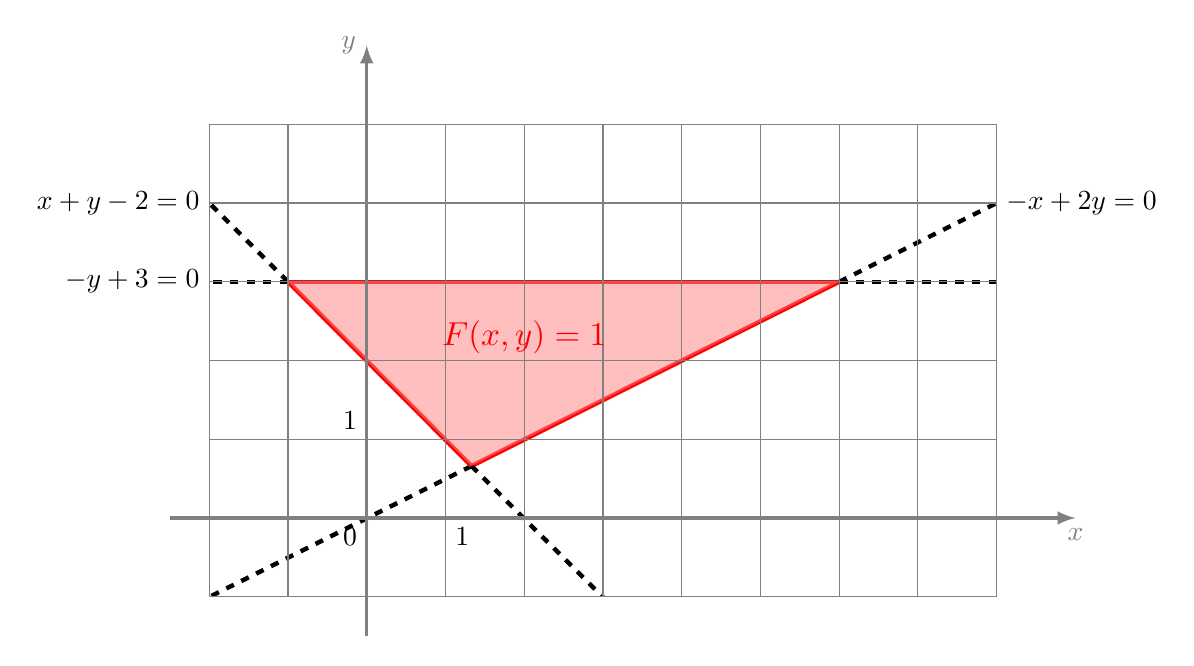
\begin{tikzpicture}[scale=1]
		
		
		
		
		\begin{scope}[even odd rule]
			\clip (-2,-1) rectangle (8,5);
			% \draw[ blue,ultra thick] (6,2) -- (-6,-2);
			% \fill[blue!20,opacity=0.5] (6,2) -- (6,6) --(-6,6) --(-6,-2)-- cycle;
			% 
			% \draw[ green!70!black,ultra thick] (-3,6) -- (3,-6);
			% \fill[ green!70!black!20,opacity=0.5] (-3,6) -- (6,6) --(6,-6) --(3,-6)-- cycle;
			
			
			
			
			\draw[ultra thick,dashed] (1.33,0.66) -- (-10,-5);
			\draw[red,ultra thick] (1.33,0.66) -- (6,3);
			\draw[ultra thick,dashed] (6,3) -- (10,5);
			
			
			\draw[ultra thick,dashed] (-1,3) -- (-7,3);
			\draw[red,ultra thick] (-1,3) -- (6,3);
			\draw[ultra thick,dashed] (6,3) -- (8,3);
			
			
			\draw[ultra thick,dashed] (-6,8) -- (-1,3);
			\draw[ red,ultra thick] (-1,3)--(1.33,0.66);
			\draw[ultra thick,dashed] (1.33,0.66)--(6,-4);
			
			
			\fill[red!50,opacity=0.5] (1.33,0.66) -- (-1,3) -- (6,3) -- cycle;
			
			
		\end{scope}
		
		
		\draw[->,>=latex, very thick,gray] (-2.5,0)--(9,0) node[below] {$x$};
		\draw[->,>=latex, very thick, gray] (0,-1.5)--(0,6) node[left] {$y$};
		\draw[gray,thin] (-2,-1) grid (8,5);
		
		
		\node[left] at (-2,4) {$x+y-2=0$};
		\node[left] at (-2,3) {$-y+3=0$};
		\node[right] at (8,4) {$-x+2y=0$};
		
		
		\node[scale=1.2,red] at (2,2.3) {$F(x,y)=1$};
		
		
		\node at (0,0) [below left] {$0$};
		\node at (1,0) [below right] {$1$};
		\node at (0,1) [above left] {$1$};
		
		
	\end{tikzpicture}
}
}
